\section{РЕАЛИЗАЦИЯ}

%Проанализировав все вышеперечисленные программы...

Таким образов в программу вошли классические алгоритмы численных методов, такие как методы матричной алгебры, методы
Ньютона и так далее. Для её написания были использованы \textit{язык программирования C++}, \textit{фреймворк QT} и система сборки
проектов \textit{CMake}. Полный список технологий и алгоритмов предоставлен на рисунке \ref{fig:stack}.
Для поиска ошибок и утечек памяти применилась связка из отладчика \textit{GDB} и профилировщика \textit{Valgrind}. 

\begin{figure}
    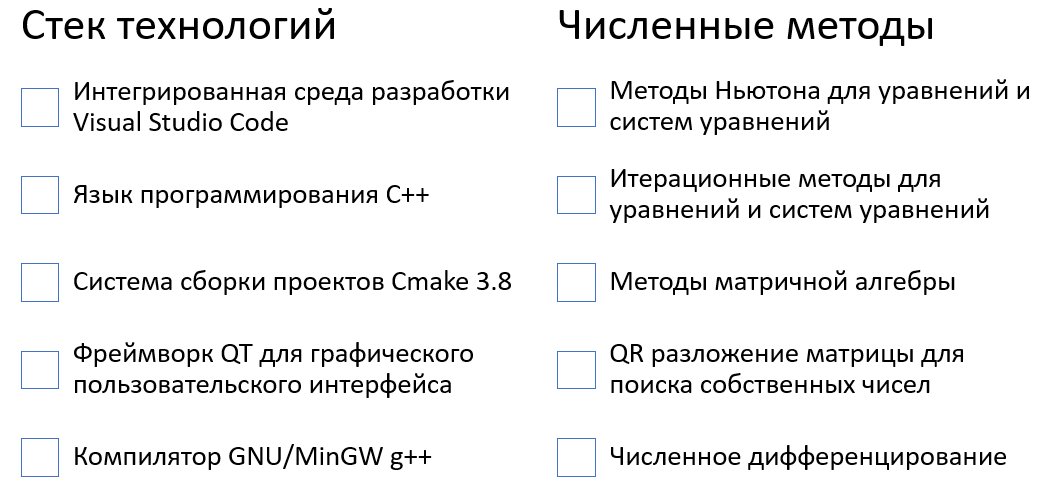
\includegraphics[width=15cm]{2-04-realisation}
    \caption{Технологии и алгоритмы}
    \label{fig:stack}
\end{figure}

Общий алгоритм работы, показан на рисунке \ref{fig:sheme}.

\begin{figure}
    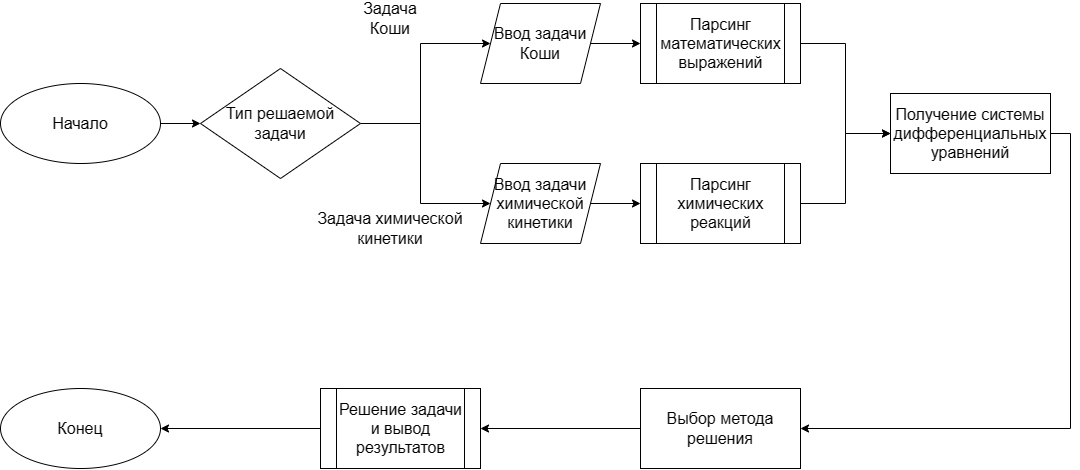
\includegraphics[width=15cm]{2-04-scheme}
    \caption{Алгоритм работы программы}
    \label{fig:sheme}
\end{figure}

Сначала выбирается тип решаемой задача, после чего всплывает форма с соответствующими текстовыми полями для ввода. После этого, в
зависимости от типа решаемой задачи, происходит обработка ввода и формирование системы дифференциальных уравнений, которые решаются
выбранным методом. Результаты работы выводятся либо на экран, либо в отдельном файле.

Для решения ОДУ был реализован большой перечень как явных так и неявных методов с различным порядком точности. Для удобства разработки
и тестирования, программа была поделена на множество отдельных модулей. Далее приведено детальное рассмотрение каждого из них.

%Для повышения порядка точности явных методов используется процедура Рунге-Ромберга, заключающаяся в повторном решении в точке с вдвое меньшим шагом и сравнении с предыдущим.

%Если погрешность сильно меньше заданной точности, что шаг интегрирования стоит уменьшить, если же больше, что увеличить.

%и вложенные методы. Неявные и их виды ()нулевая строка, нулевой столбец, диагональные, полные) параллельные

\subsection{Общие алгоритмы и структуры}

В данном подразделе перечислены основные алгоритмы и структуры, которые использовались в остальных модулях. Сюда вошли алгоритмы
LU-разложения матрицы, QR алгоритм нахождения собственных чисел матрицы, алгоритмы дифференцирования с разным порядком точности. Для
работы с таблицами Бутчера и алгоритмами решения СЛАУ был реализован собственный класс матрицы с базовой матричной алгеброй.

\textbf{LU алгоритм}

\textbf{QR алгоритм}

\textbf{Дифференцирование}

\subsection{Вычисление жёсткости}

Для вычисления числа жёсткости по формуле \ref{eq:tough} нужно составить матрицу-систему и найти её собственные числа.

Коэффициентом жёсткости задачи называется отношение максимального модуля действительной части собственных чисел матрицы системы к
минимальной при условии, что все действительные части собственных чисел меньше нуля.

Для вычисления коэффициента жёсткости сначала по данной задаче строится матрица-система. Собственные числа данной матрицы находятся
при помощи алгоритма QR-разложения.

%дополнительные методы ()кью-ар
%методы решения слау

%методы решения

%Для неявных методов используются алгоритмы итераций Ньютона, Зейделя и простой итерации.

%алгоритмы работы с матрицами

%Кью-Ар разложение 

%хоть метод ньютона и второго порядка но применим и для методов

\subsection{Парсер математических выражений}

При режиме работы с задачей Коши от пользователя требуется ввести задачу и аналитическое решение (при наличии). 

Для обработки строки с задачей был реализован парсер математических выражений. Проводится лексический анализ строки и строится дерево
математических выражений, содержащее функции в качестве узлов и числовые константы с переменными в качестве листьев.

Реализацияв виде дерева была выбрана по нескольким причинам:

\begin{itemize}
    \item лёгкость в реализации,
    \item простота в расширении функционала,
    \item некоторые операции (поиск коеффициентов при переменной, выделение поддерева и т.д.) легче выполнять при работе с деревом.
\end{itemize}

Интерфейс парсера позволяет использовать его как функтор, принимающий либо одну переменную, либо массив переменных. Реализована поддержка
базовых функций и числовых констант. Так же есть возможность добавления пользовательских параметров и констант.

Рисунок \ref{src:FuncMaker} показывает листинг с примерами использования парсера:

\begin{figure}
    \lstinputlisting[language=C++]{inc/Code/FuncMaker.cpp}
    \caption{Пример использования парсера}
    \label{src:FuncMaker}
\end{figure}

Для сравнения эффективности реализации было проведено тестирование на модельных функциях с использованием парсера и обычных
статических функций. Сравнения по времени приведены в таблице \ref{tab:Banchmark}:

\begin{table}    
    \caption{Таблица сравнения методов}
    \begin{tabularx}{\textwidth}{|X|c|c|}
    \hline
    Уравнение & Статическая функция (ms) & Парсера (ms)\\
    \hline
    $x + 2$ & 18 & 35\\
    \hline
    $\sin(\cos(x)) + \cos(\cos(x))$ & 253 & 492\\
    \hline
    $\sin(-x) + \ln(e^{10}) + \arccos((-1)^x)$ & 623 & 1007\\
    \hline
    $\dfrac{(11 - x^3 (3x - 8))}{(12(x - 2)^2 (x - 3))}$ & 23 & 172\\
    \hline
    $x\exp(\dfrac{1}{x})$ & 29 & 109\\
    \hline
    $\exp(x\sin(\ln(x)) + x)$ & 393 & 385\\
    \hline
    $\dfrac{1}{4}x^3 - \dfrac{1}{x}$ & 22 & 108\\
    \hline
    $1 + \ln(abs(x))$ & 40 & 65\\
    \hline
    $\cos(\sqrt{4x}) + \sin(\sqrt{4x})$ & 303 & 349\\
    \hline
    $abs(x)^\frac{3}{2}$ & 249 & 293\\
    \hline
    \end{tabularx}
    \label{tab:Banchmark}
\end{table}

На данной таблице видно, что парсер уступает по скорости обычным функциям в 1.5-2 раза. Это связано с тем, что при работе с деревом
приходится проходить по указателям к нижним узлам, что сильно замедляет работу алгоритма.
Так же была протестирована реализация парсинга математических выражений при помощи обратной польской записи, однако она давала небольшой
выигрыш по времени при урезанном функционале.

\subsection{Реализация методов решения}

Как уже говорилось выше, все методы семейства Рунге-Кутты можно представить в виде таблиц Бутчера. В связи с этим появилась идея
реализовать алгоритм, принимающий задачу и таблицу Бутчера и возвращающий решение в виде таблицы. Благодаря этому алгоритму добавлять
новые методы не вызывает никаких сложностей. Используемые методы перечислены на рисунке \ref{fig:SolveMethods}.
Всего в данной работе используется 62 схемы с 1 по 6 порядок точности.

\begin{figure}
    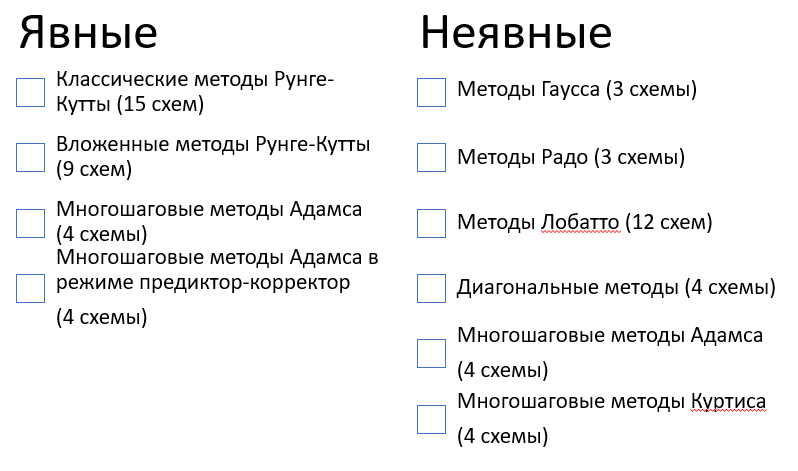
\includegraphics[width=15cm]{2-04-methods}
    \caption{Методы решения}
    \label{fig:SolveMethods}
\end{figure}

По желанию пользователя можно добавить другой метод при помощи специального конструктора.

\subsection{Форма для ввода/вывода}

Для ввода задачи была реализована специальная форма с использованием фреймворка QT. Её внешний вид представлен на рисунке \ref{fig:forma}.

\begin{figure}
    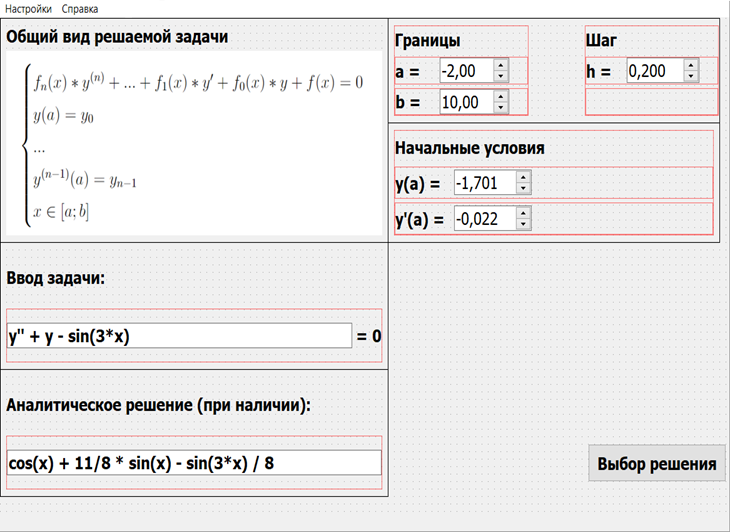
\includegraphics[width=15cm]{2-04-forma}
    \caption{Вид интерфейса для ввода задачи Коши}
    \label{fig:forma}
\end{figure}

После ввода задачи, аналитического решения (при наличии), начальных условий и границ интегрирования требуется выбрать метод решения.
Перед выбором решения идёт анализ задачи на жёсткость и если число жёсткости задачи велико ($> 100$), то выбор методов ограничивается
неявными, иначе выбор методов не ограничивается. Результаты вичислений либо сохраняются в отдельном файле, либо выводятся на экран.

\subsection{Генерация отчёта}

При генерации отчёта учитывается количество уравнений, тип решаемой задачи, количество шагов интегрирования. При решении задач химической
кинетики аналитическое решение не вводится. Отдельно выводятся графики изменения плотности и температуры. В обоих типах задач при
большом количестве точек их число уменьшается в несколько раз (оставляется каждая вторая или каждая третья). На рисунке \ref{fig:report}
показан пример одной страницы отчёта.

\begin{figure}
    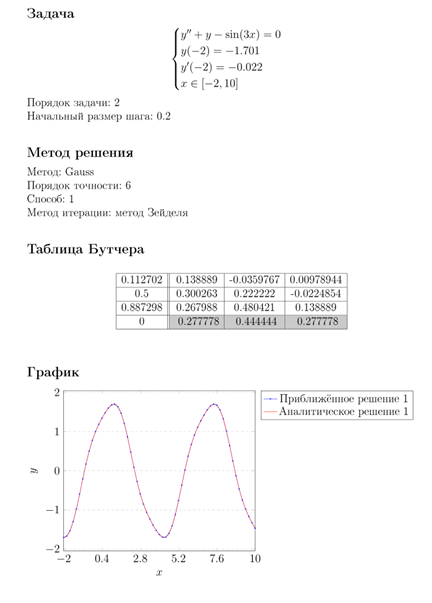
\includegraphics[width=10cm]{2-04-report}
    \caption{Пример страницы отчёта}
    \label{fig:report}
\end{figure}

Для версии программы без интерфейса отчёт выводится либо в текстовом виде, либо в TeX-файле.
